\documentclass[tikz,border=5pt]{standalone}
\usepackage{amsmath}
\usepackage{pgfplots}
\pgfplotsset{compat=1.18}
\usetikzlibrary{arrows.meta,calc}
\definecolor{ink}{HTML}{16324F}
\definecolor{teal}{HTML}{168A88}
\definecolor{gold}{HTML}{D9892B}
\definecolor{redq}{HTML}{B84A4A}
\begin{document}
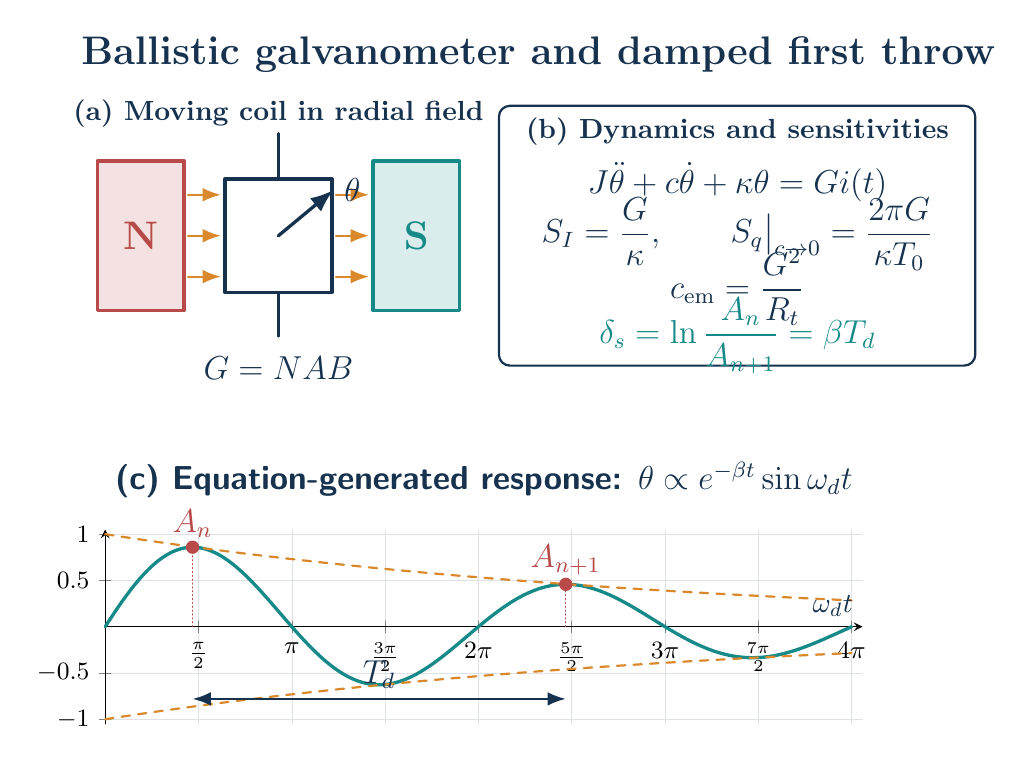
\begin{tikzpicture}[font=\large\sffamily,>=Latex,line cap=round,line join=round]
  \node[font=\bfseries\Large,ink] at (6.1,8.75)
    {Ballistic galvanometer and damped first throw};

  \begin{scope}[shift={(.45,4.75)}]
    \node[font=\bfseries,ink] at (2.35,3.25) {(a) Moving coil in radial field};
    \fill[redq!16] (.05,.75) rectangle (1.15,2.65);
    \draw[redq,very thick] (.05,.75) rectangle (1.15,2.65);
    \node[redq,font=\bfseries\Large] at (.60,1.70) {N};
    \fill[teal!16] (3.55,.75) rectangle (4.65,2.65);
    \draw[teal,very thick] (3.55,.75) rectangle (4.65,2.65);
    \node[teal,font=\bfseries\Large] at (4.10,1.70) {S};
    \draw[ink,very thick] (1.67,.98) rectangle (3.03,2.42);
    \draw[ink,thick] (2.35,2.42)--(2.35,3.0);
    \draw[ink,thick] (2.35,.98)--(2.35,.42);
    \foreach \y in {1.18,1.70,2.22}{
      \draw[->,gold,thick] (1.2,\y)--(1.62,\y);
      \draw[->,gold,thick] (3.08,\y)--(3.5,\y);
    }
    \draw[->,ink,very thick] (2.35,1.70)--(3.05,2.28) node[right] {$\theta$};
    \node[ink] at (2.35,.02) {$G=NAB$};
  \end{scope}

  \begin{scope}[shift={(5.55,4.75)}]
    \draw[ink,thick,rounded corners] (.05,.05) rectangle (6.1,3.35);
    \node[font=\bfseries,ink] at (3.08,3.02) {(b) Dynamics and sensitivities};
    \node[ink] at (3.08,2.38)
      {$\displaystyle J\ddot\theta+c\dot\theta+\kappa\theta=Gi(t)$};
    \node[ink] at (3.08,1.72)
      {$\displaystyle S_I=\frac{G}{\kappa},\qquad
        S_q\big|_{c\to0}=\frac{2\pi G}{\kappa T_0}$};
    \node[ink] at (3.08,1.04)
      {$\displaystyle c_{\rm em}=\frac{G^2}{R_t}$};
    \node[teal] at (3.08,.43)
      {$\displaystyle \delta_s=\ln\frac{A_n}{A_{n+1}}=\beta T_d$};
  \end{scope}

  \begin{axis}[
    at={(.6cm,.25cm)},anchor=south west,
    width=11.2cm,height=4.05cm,
    xmin=0,xmax=12.75,ymin=-1.05,ymax=1.05,
    axis lines=middle,
    xlabel={$\omega_dt$},ylabel={},
    xtick={0,1.571,3.142,4.712,6.283,7.854,9.425,10.996,12.566},
    xticklabels={$0$,$\frac\pi2$,$\pi$,$\frac{3\pi}2$,$2\pi$,$\frac{5\pi}2$,$3\pi$,$\frac{7\pi}2$,$4\pi$},
    ytick={-1,-.5,0,.5,1},
    grid=both,grid style={draw=ink!14,line width=.2pt},
    tick label style={font=\small},
    label style={font=\normalsize,ink},
    title={\bfseries (c) Equation-generated response:
      \(\theta\propto e^{-\beta t}\sin\omega_dt\)},
    title style={ink,yshift=2pt},
    clip=false
  ]
    \addplot[teal,very thick,domain=0:12.566,samples=500]
      {exp(-.1*x)*sin(deg(x))};
    \addplot[gold,thick,dashed,domain=0:12.566,samples=220] {exp(-.1*x)};
    \addplot[gold,thick,dashed,domain=0:12.566,samples=220] {-exp(-.1*x)};
    \addplot[only marks,mark=*,mark size=2.2pt,redq]
      coordinates {(1.471,.859) (7.754,.458)};
    \draw[redq,densely dotted] (axis cs:1.471,0)--(axis cs:1.471,.859);
    \draw[redq,densely dotted] (axis cs:7.754,0)--(axis cs:7.754,.458);
    \node[redq,above] at (axis cs:1.471,.859) {$A_n$};
    \node[redq,above] at (axis cs:7.754,.458) {$A_{n+1}$};
    \draw[<->,ink,thick] (axis cs:1.471,-.78)--(axis cs:7.754,-.78)
      node[midway,above] {$T_d$};
  \end{axis}
\end{tikzpicture}
\end{document}
